%%%%%%%%%%%%%%%%%%%%%%%%%%%%%%%%%%%%%%%%%
% Short Sectioned Assignment LaTeX Template Version 1.0 (5/5/12)
% This template has been downloaded from: http://www.LaTeXTemplates.com
% Original author:  Frits Wenneker (http://www.howtotex.com)
% License: CC BY-NC-SA 3.0 (http://creativecommons.org/licenses/by-nc-sa/3.0/)
%%%%%%%%%%%%%%%%%%%%%%%%%%%%%%%%%%%%%%%%%

%----------------------------------------------------------------------------------------
%	PACKAGES AND OTHER DOCUMENT CONFIGURATIONS
%----------------------------------------------------------------------------------------

\documentclass[paper=a4, fontsize=11pt]{scrartcl} % A4 paper and 11pt font size

% ---- Entrada y salida de texto -----

\usepackage[T1]{fontenc} % Use 8-bit encoding that has 256 glyphs
\usepackage[utf8]{inputenc}
%\usepackage{fourier} % Use the Adobe Utopia font for the document - comment this line to return to the LaTeX default

% ---- Idioma --------

\usepackage[spanish, es-tabla]{babel} % Selecciona el español para palabras introducidas automáticamente, p.ej. "septiembre" en la fecha y especifica que se use la palabra Tabla en vez de Cuadro

\usepackage{fancyhdr}

% ---- Otros paquetes ----

\usepackage{amsmath,amsfonts,amsthm} % Math packages
%\usepackage{graphics,graphicx, floatrow} %para incluir imágenes y notas en las imágenes
\usepackage{graphics,graphicx, float} %para incluir imágenes y colocarlas

% Para hacer tablas comlejas
%\usepackage{multirow}
%\usepackage{threeparttable}

%\usepackage{sectsty} % Allows customizing section commands
%\allsectionsfont{\centering \normalfont\scshape} % Make all sections centered, the default font and small caps

\usepackage{fancyhdr} % Custom headers and footers
\usepackage{url}
%\usepackage{hyperref}
\pagestyle{fancyplain} % Makes all pages in the document conform to the custom headers and footers
\fancyhead{} % No page header - if you want one, create it in the same way as the footers below
\fancyfoot[L]{} % Empty left footer
\fancyfoot[C]{} % Empty center footer
\fancyfoot[R]{\thepage} % Page numbering for right footer
\renewcommand{\headrulewidth}{0pt} % Remove header underlines
\renewcommand{\footrulewidth}{0pt} % Remove footer underlines
\setlength{\headheight}{13.6pt} % Customize the height of the header

\numberwithin{equation}{section} % Number equations within sections (i.e. 1.1, 1.2, 2.1, 2.2 instead of 1, 2, 3, 4)
\numberwithin{figure}{section} % Number figures within sections (i.e. 1.1, 1.2, 2.1, 2.2 instead of 1, 2, 3, 4)
\numberwithin{table}{section} % Number tables within sections (i.e. 1.1, 1.2, 2.1, 2.2 instead of 1, 2, 3, 4)

\setlength\parindent{0pt} % Removes all indentation from paragraphs - comment this line for an assignment with lots of text

\newcommand{\horrule}[1]{\rule{\linewidth}{#1}} % Create horizontal rule command with 1 argument of height

\usepackage{booktabs}




%----------------------------------------------------------------------------------------
%	TÍTULO Y DATOS DEL ALUMNO
%----------------------------------------------------------------------------------------

\title{	
\normalfont \normalsize 
\textsc{{\bf Metaheurísticas (2014-2015)} \\ Grado en Ingeniería Informática \\ Universidad de Granada} \\ [25pt] % Your university, school and/or department name(s)
\horrule{0.5pt} \\[0.4cm] % Thin top horizontal rule
\huge  Práctica 4 - Optimización basada en Colonias de Hormigas \\ % The assignment title
\horrule{2pt} \\[0.5cm] % Thick bottom horizontal rule
}

\author{Ignacio Martín Requena} % Nombre y apellidos

\date{\normalsize\today} % Incluye la fecha actual

%----------------------------------------------------------------------------------------
% DOCUMENTO
%----------------------------------------------------------------------------------------
\usepackage{graphicx}
\usepackage{listings}
\usepackage{color}
\definecolor{gray97}{gray}{.97}
\definecolor{gray75}{gray}{.75}
\definecolor{gray45}{gray}{.45}
 

\lstset{ frame=Ltb,
     framerule=0pt,
     aboveskip=0.5cm,
     framextopmargin=3pt,
     framexbottommargin=3pt,
     framexleftmargin=0.4cm,
     framesep=0pt,
     rulesep=.4pt,
     backgroundcolor=\color{gray97},
     rulesepcolor=\color{black},
     %
     stringstyle=\ttfamily,
     showstringspaces = false,
     basicstyle=\small\ttfamily,
     commentstyle=\color{gray45},
     keywordstyle=\bfseries,
     %
     numbers=left,
     numbersep=15pt,
     numberstyle=\tiny,
     numberfirstline = false,
     breaklines=true,
   }
 


\lstdefinestyle{consola}
   {basicstyle=\scriptsize\bf\ttfamily,
    backgroundcolor=\color{gray75},
   }
 
\lstdefinestyle{C}
   {language=C,
   }



\begin{document}

\maketitle % Muestra el Título

\newpage %inserta un salto de página

\tableofcontents % para generar el índice de contenidos

\listoffigures

%\listoftables

\newpage




%----------------------------------------------------------------------------------------
%	Cuestion 1
%----------------------------------------------------------------------------------------
\section{Descripción del problema}
El problema de la asignación cuadrática (QAP) es un problema clásico en teoría de localización. En éste se trata de asignar N unidades a una cantidad N de sitios o localizaciones en donde se considera un costo asociado a cada una de las asignaciones. Este costo dependerá de las distancias y flujo entre unidades, además de un costo adicional por asignar cierta unidad a una localización específica. De este modo se buscará que este costo, en función de la distancia y flujo, sea mínimo.

Este problema tiene muchas aplicaciones, como el diseño de hospitales donde se pretende que los médicos recorran la menor distancia posible dependiendo de su especialidad, procesos de comunicaciones, diseño de teclados de un ordenador, diseño de circuitos eléctricos, diseño de terminarles en aeropuertos y, en general, todo aquel problema de optimización de trayectorias y localizaciones que posea un espacio de búsqueda considerablemente grande. 

%----------------------------------------------------------------------------------------
%	Cuestion 2
%----------------------------------------------------------------------------------------
\section{Descripción de los algoritmos empleados}

En esta sección vamos a especificar las componentes comunes a todos los algoritmos empleados para la resolución del problema:

\begin{itemize}
	\item \textbf{Representación de la solución: }
	
	La forma más conveniente considerada para representar las soluciones es a través de las permutaciones de un conjunto. Esto quiere decir que si por ejemplo el problema tiene, por ejemplo, tamaño cuatro, una posible solución al problema sería N = \{1,4,2,3\}. De esta forma, si interpretamos los índices de este conjunto como las unidades, y el valor del índice como su localización, la localización 3 estaría asignada a la unidad 1, la 4 a la 2 y así sucesivamente.
	
	\subsection{Metaheurísticas y funciones que ayudan al desarrollo de la práctica}
	
	\item \textbf{Función objetivo:}
	
	Dado que el objetivo del problema es la minimización del costo total de todas las posibles soluciones, la función objetivo vendrá definida matemáticamente como:
	
	\begin{figure}[H]
		\centering
		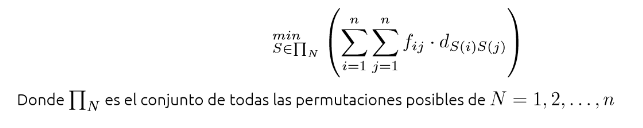
\includegraphics[scale=1.0]{Screenshot_2.png}
		\caption{Función objetivo}
		\label{}
	\end{figure}
	\newpage
	En forma de pseudicódigo nuestra función objetivo sería:
	
	\begin{lstlisting}[language=SH]
inicializamos el costo a 0
para cada fila de las matrices de distancia y flujo
	para cada posicion de las matrices de distancia y flujo
		costo += flujo[i][j] * distancia[[i]][sol[j]];

	\end{lstlisting}
	

			\item \textbf{Función BL:}
		Este algoritmo se compone de dos partes: La creación de la máscara Don't Look Bite y el propio algoritmo de búsqueda

			Una representación en pseudicódigo de esta función sería:
			
					\begin{lstlisting}[language=SH]
					
Inicializamos DLB a 0, y con un tamao igual que el del problema
Creamos una variable para saber cuando parar de iterar
Mientras se pueda seguir iterando
	Para i=1...n
		si DLB[i] == 0
			Para j=1...n
				si costo factorizado actual menor que 0
					intercambiamos localizaciones de solucion actual
					dlb[i] = dlb[j] = 0;
					paramos de iterar
			si podemos seguir iterando
				dlb[i] = 1;
Devolver estado actual
					\end{lstlisting}

Además, la busqueda local usa las siguientes funciones:
\newpage
	\item \textbf{Función factorizar:}
	
	Con el fin de aumentar la eficiencia y el tiempo de ejecución de nuestros algoritmos se implementa la función factorizar, que nos calcula la diferencia de costo entre una solución y otra, de esta forma evitamos el tener que calcular el costo de una solución de principio a fin.
	
	En forma de pseudicódigo nuestra función factorizar sería:
	
	\begin{lstlisting}[language=SH]
	
    inicializamos una variable suma a 0
    
    desde i=0 hasta N hacer
	    si i no coincide con ninguna de las localizaciones a inercambiar
		    realizar el coste del movimiento de intercambio como la sumatoria de la diferencia de todas las distancias nuevas menos las viejas multiplicadas por el flujo
	
	\end{lstlisting}

	\item \textbf{Función generar vecino:}	
	Esta función calcula una solución vecina a partir de una solución actual y dos posiciones a intercambiar.
	
	En forma de pseudicódigo nuestra función "swap" sería:
	
	\begin{lstlisting}[language=SH]

Crear un vector para guardar la nueva solucion
Para cada elemento de la solucion actual
	Copiar en el nuevo vector solucion
Guardar en una variable el valor de la posicion a intercambiar
Cambiar dicho valor por el contenido en la otra posicion
Asignar a la otra posicion el valor guardado en el paso 5 
Actualizar el costo de la solucion como el costo de la solucion inicial mas el factorizado
Devolver la nueva solucion

	\end{lstlisting}
	\newpage
		\item \textbf{Función generar solución aleatoria:}	
		Esta función calcula una solución inicial generada aleatoriamente.
		
		En forma de pseudicódigo nuestra función "getSolAleatoria" sería:
		
		\begin{lstlisting}[language=SH]
		
Creamos un vector de enteros con el tamano de las matrices de flujo o distancia
Para cada posicion del vector creado
	Generamos un numero aleatorio compremndido entre la posicion actual y el tamano del vector
	Introducimos este numero en el vector de soluciones iniciales
Calculamos el costo de la solucion inicial
Devolvemos la solucion y su costo
		\end{lstlisting}
		
		\subsection{Funciones que toman parte en el proceso de contrucción de SCH y SHMM}
			\item \textbf{Descripción en pseudocódigo del cálculo de la información heurística:}
	
	\begin{lstlisting}[language=SH]
	
para cada elemento de la lista de candidatos
        incializar variable heuristica
        para cada elemento de la lista de candidatos
            HeuristicaC = suma de la distancia de cada par de candidatos
            heuristica de candidato = 1/HeuristicaC
        
	
	\end{lstlisting}
\newpage		
		\item \textbf{Proceso constructivo para generar soluciones:}
		
		Casi todo el proceso a partir del cual se generan las soluciones se realiza en la función ``avanzar'' de código adjunto en esta documentación. La descripción de esta función en pseudicódigo es:
		
		\begin{lstlisting}[language=SH]
		
Creamos e inicializamos una lista de valores binarios para las localizaciones asignadas/sin asignar
Buscamos la lista de candidatos, es decir,las localizaciones sin asignar (con valor 0)
Calculamos la heuristica de cada candidato segun lo descrito en el apartado anterior
Aplicamos la regla de transicion
Lanzamos un valor aleatorio
Si es menor o igual que q0
	Elegir el mejor de los candidatos
Si no
	Hacer ruleta para cada candidato
	Asignamos la localizacion seleccionada a la hormiga (indice de la solucion de la hormiga actual = localizacion)
		\end{lstlisting}

\end{itemize} 

\newpage		
%----------------------------------------------------------------------------------------
%	Cuestion 3
%----------------------------------------------------------------------------------------
\section{Descripción del esquema de búsqueda y las operaciones de cada algoritmo}	
		
		\subsection{SCH}
		
		El algoritmo principal el SCH con el que se ha elavorado la práctica ha sido:
		
	\begin{lstlisting}[language=SH]
					
Definimos los parametros del algoritmo (alpha, beta, q0...)
Ordenamos el vector potencial de flujo de menor a mayor
Creamos e inicializamos la matriz de feromona
Hasta numero_evaluaciones = MAX_EVALUACIONES
	Creamos e inicializamos los caminos que van a recorrer las hormigas
	
   //Construimos los caminos de cada hormiga
    Para cada paso (pasos = tamano problema)
		Para cada hormiga
			Lamar a la funcion avanzar para generar nuevas soluciones

    Calcular el costo de cada camino
	Hacer busqueda local al mejor camino encontrado
	
   //Actualizar la feromona 
    Para cada unidad de feromona
            feromona[i][mejorencontrada->sol[i]] = ((1.0-evaporacion_global)*feromona[i][mejorencontrada->sol[i]]) + (evaporacion_global / mejorencontrada->costo)


    Devolver mejor solucion encontrada


	\end{lstlisting}
	
	
		\newpage
		\subsection{SHMM}
		La metaheuristica SHMM realizada en la práctica en forma de pseudocódigo es:
		
\begin{lstlisting}[language=SH]
	
	Generamos una solucion aleatoria
	Calculamos la matriz de potencial de flujo
	Concretamos los parametros necearios para el algoritmo (q0, evaporacion, alpha, beta, t_max y t_min)
	Crear e inicializar con t_max la matriz de feromonas
	
	Mientras no se llegue al maximo de evaluaciones
		Creamos la estructura de datos para guardar los caminos de las hormigas
		Llamamos a la funcion avanzar para cada hormiga y en cada paso (de esta forma todas las hormigas avanzan a la vez)
		Calculamos el costo de cada hormiga
		Hacemos una busqueda local a la mejor solucion encontrada
		Si la mejor encontrada supera a la mejor hasta ahora nos quedamos con ella y actualizamos los valores de t_max y t_min de la forma: (Los reinicializamos)
			t_max = 1.0/(evaporacion_global * mejorencontrada->costo)
			t_min = t_max/500.0
		//Simulamos la evaporacion de las feromonas
		Para cada elemento de feromona
			Para cada posicion dentro de feromona
				feromona[i][j] = feromona[i][j] *(1.0 - coeficiente de evaporacion global)
		
		Buscamos la peor solucion
		
		Para cada elemento de feromona en el que este la peor solucion hacer
			feromona[i][caminos[idx]->sol[i]] = ((1.0-evaporacion_global)*feromona[i][caminos[idx]->sol[i]]) + (1.0 / caminos[idx]->costo)
		
		Si se supera el t_maximo por los decimales, truncar
		
		
	Devolver la mejor solucion encontrada
	\end{lstlisting}
		
		
		
		
%----------------------------------------------------------------------------------------
%	Cuestion 4
%----------------------------------------------------------------------------------------
\newpage
\section{Algoritmo de comparación: Greedy}
Este algoritmo no hace mas que calcular los potenciales de cada unidad y de cada localización, los ordena y asigna el de mayor flujo al de menor distancia.

En pseudocódigo sería algo como:

\begin{lstlisting}[language=SH]
Declaramos un estado solucion
Ordenamos por flujo la matriz de flujo y por distancia la de distancia
Para i=0..n
	Asignamos al elemento determinado por flujo del estado solucion el elemento distancia (podemos hacerlo asi ya que hemos ordenado los vectores previamente.)
Asignamos el costo de la solucion
Devolvemos el estado

\end{lstlisting}

%----------------------------------------------------------------------------------------
%	Cuestion 5
%----------------------------------------------------------------------------------------
\section{Procedimiento considerado para desarrollar la práctica}
Para la realización de esta práctica me he basado en una implementación que he encontrado por internet\footnote{\url{http://quadratic-assignation.googlecode.com/svn-history/r44/trunk/qap.cpp}} dado que me ha resultado facil de entender y elegante, sobre todo por la utilización del struc de Estados. Aun así la modificación a este codigo ha sido casi entera y solo se han usado las estructuras y la lectura de los ficheros que el enlace proporciona. Me ha resultado de gran ayuda ya que tenía algunos operadores de copia implementados. El resto de ayudas han venido sobre todo de mano de los apuntes de clase, del guion de prácticas o de charlas con compañeros de clase.
\newpage
%----------------------------------------------------------------------------------------
%	Cuestion 6
%----------------------------------------------------------------------------------------
\section{Experimentos y análisis de los resultados}

Los problemas que he empelado han sido los mismos que los que vienen en la plantilla que se nos proporciona. Para cada caso, los parámetros para su ejecución son:

./qap <Metaheuristica> <archivo de entrada> <semilla>\\

donde metaheurística indica la metaheurística a usar:\\
1) Greedy\\
2) SCH\\
3) SHMM\\


La semilla usada ha sido la \textbf{4312365} 

A continuación se muestran las tablas con los resultados obtenidos:

\begin{figure}[H]
\centering
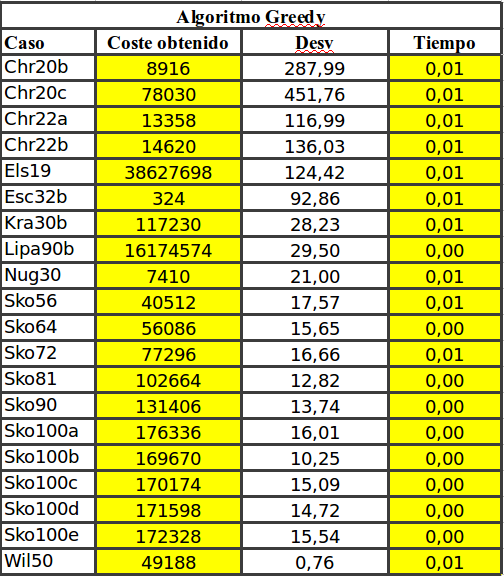
\includegraphics[scale=.60]{greedy.png}
\caption{Resultados algoritmo Greedy}
\label{}
\end{figure}


\begin{figure}[H]
\centering
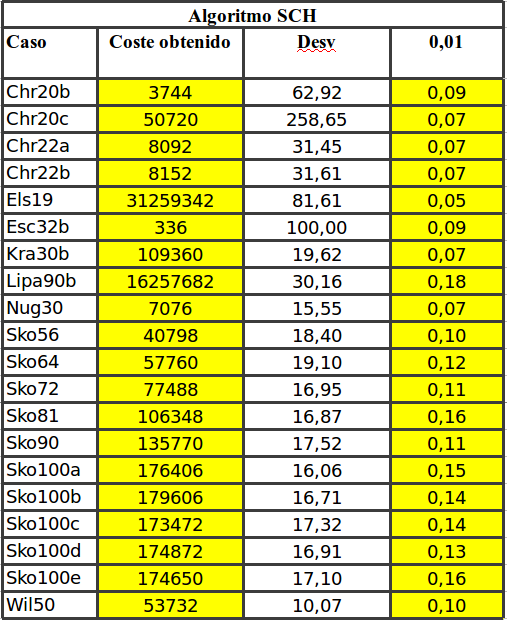
\includegraphics[scale=.60]{sch.png}
\caption{Resultados algoritmo SCH}
\label{}
\end{figure}


\begin{figure}[H]
\centering
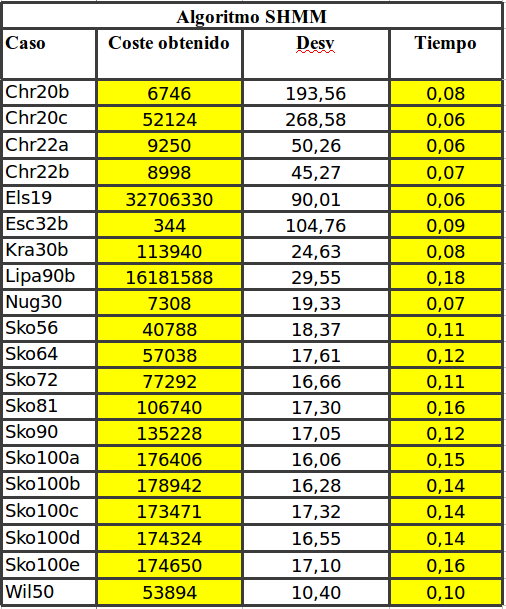
\includegraphics[scale=.60]{scmm.png}
\caption{Resultados algoritmo SHMM}
\label{}
\end{figure}



\begin{figure}[H]
\centering
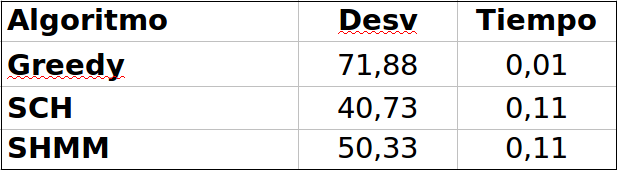
\includegraphics[scale=.40]{total.png}
\caption{Comparación de los algoritmos}
\label{}
\end{figure}

En este caso, aunque pareciera que el proceso busqueda basado en metaheurísticas de colonias de hormigas fuera a dar buenos resultados no ha resultado ser el mejor calculo. Una cosa que aún me inquieta es el hecho de que tarde tan poco en realizar las operaciones (al ser una metaheurística basada en poblaciones el proceso de cálculo debería llevar más tiempo en realizarse, en las tablas no llegan ni a un segundo el tiempo de calculo). Supongo que aun quedaría mucho por optimizar este método para que diera buenos resultados, por lo que no hay que subestimarlo, seguro que puede dar soluciones mucho mejores que las encontradas actualmente.\\

A raíz de los resultados tan poco cercanos a los óptimos se me ocurrió modificar la metaheurística para añadirle mas poder de intesificación, es decir, definir un umbral a partir del cual se le aplicara busqueda local a todas las hormigas, pero en vez de mejorar las soluciones las empeoraba así que decidí no incluirlo en la práctica al no aportar nada a la mejora de la solución.\\



\end{document}